%!TEX root = main.tex
\chapter{Polymers}

Many of the most important molecules in biology are polymers:
DNA and RNA encode genetic information in the order of bases, proteins are polypeptides, and the cytoskeleton provides structure and stability to cells.
We will discuss properties of
\begin{itemize}
	\item single stranded RNA and DNA
	\item double stranded DNA
	\item cyctoskeletal filaments
\end{itemize}
The microscopic properties of these different polymers depend on their molecular structure, but on larger scales their behavior is governed by a few mesoscopic parameters such as stiffness, charge, self-interaction, and cross-linking.
These large scale properties can be studied with abstract models.
Polymers are also ubiquitous in our every day life: rubber, plastics, many textiles, and many food items are made from polymers.
These materials have often surprising properties which can be understood with mathematical models.
The physical properties of polymers are dictated by a trade-off between entropy and energy: Bending a polymer typically requires energy, but there are many more bent and coiled confirmations than straight confirmations.
Depending on how this trade-off plays out, we expect these polymer configurations to vary from straight rods to messy coils.


\begin{figure}[tb]
	\centering
	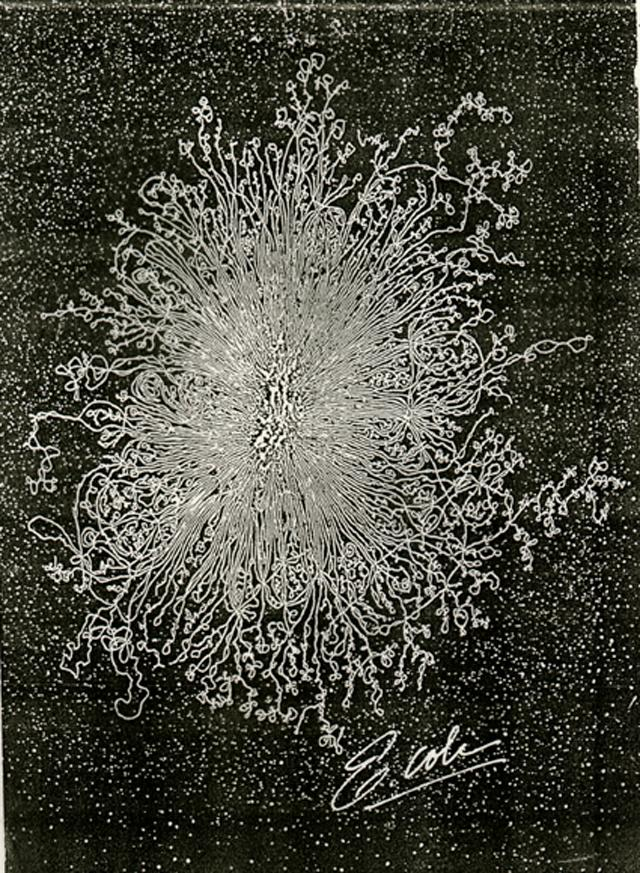
\includegraphics[width=0.44\textwidth]{lysed_ecoli.jpg}
	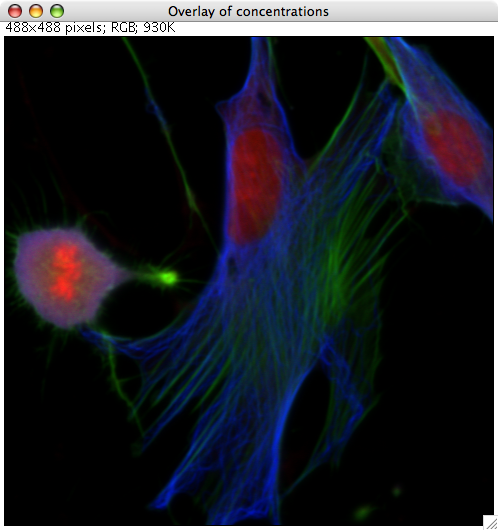
\includegraphics[width=0.55\textwidth]{figures/cytosceleton_RGB.png}
	\caption{Left: DNA from a lysed E coli (source: http://i.imgur.com/kaFF3.jpg) reveals its long filamentous structure. Right: The cytosceleton provides structure and rigity to the cell. Actin filaments are shown in green, tubulin in blue, DNA in red.}
	\label{fig:polymer_overview}
\end{figure}

\section{Polymers as information carriers}
DNA and RNA are hetero-polymers -- long chains of similar but not identical subunits.
These subunits are covalently strung together and their order encodes information -- much like letters in a text.
To full-fill their function, these polymers need to be
\begin{itemize}
	\item sufficiently stable
	\item accessible
	\item allow for accurate synthesis and copying
\end{itemize}
These requirements are more severe for DNA than for mRNA, which serves mostly as an intermediate message.

\section{Proteins are polymers}
Proteins are folded polypeptide chains (hetero-polymers as above).
But instead of storing or transmitting information, the order of amino acids in the polypeptide determines the fold and function of the protein.
The linear order of the amino acids is not crucial for the final product, but likely essential in the folding process: detached amino acids in solution would never assemble into a globular protein.
Protein folding and denaturation was covered at great length by Sebastian Hiller and we won't discuss this again here.

\section{Polymers as structural elements}
The aspects of polymer that we'll study in most detail here is how cells use them to exert force and control shape.
The three main classes of filaments of the cytoskeleton are
\begin{itemize}
	\item actin filaments
	\item microtubuli
	\item intermediate filaments
\end{itemize}
Actin and microtubuli are made from small globular proteins that associate non-covalently to form long filaments.
Intermediate filaments are made from ``coiled-coil'' subunits that make them exceptionally extendable.

These different filaments have very different mechanical properties.
These properties can -- to a large extent -- be understood using physical reasoning on how monomers assemble into filaments, how long they are, and how filaments are cross-linked to each other.

\begin{figure}[tb]
	\centering
	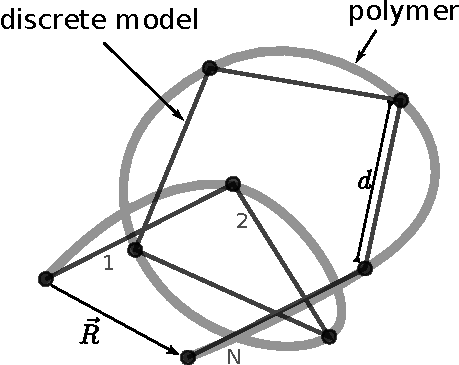
\includegraphics[width=0.43\textwidth]{figures/jointed_chain.pdf}
	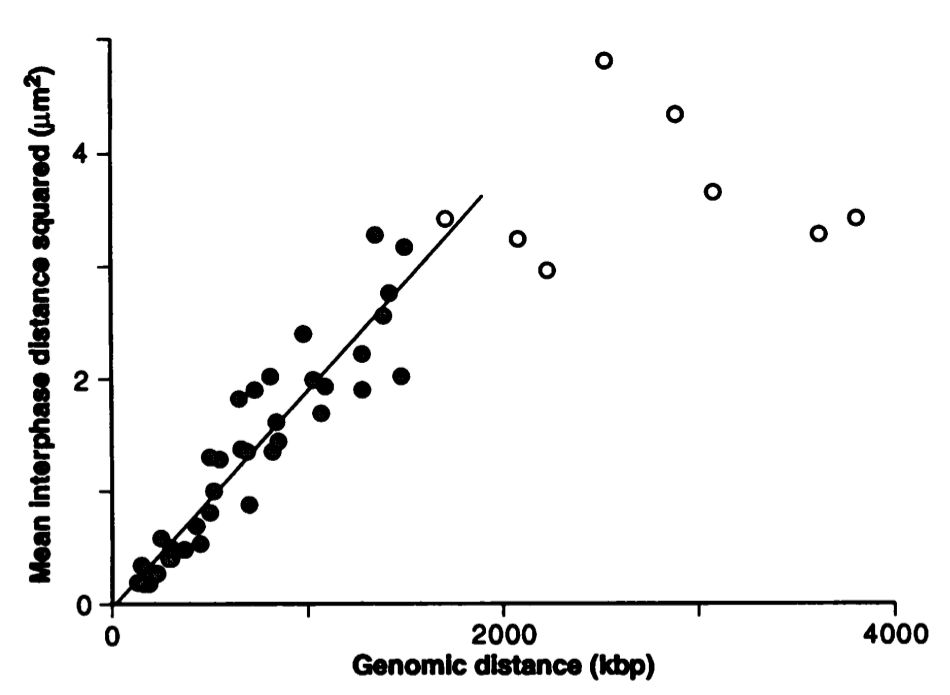
\includegraphics[width=0.55\textwidth]{figures/Genome_conformation_van_den_Engh.png}
	\caption{Illustration of the simple discrete polymer models.
	Right: Mean squared separation of chromosomal markers as a function of their genomic distance. Data from \citet{engh_estimating_1992}.}
	\label{fig:polymer_models}
\end{figure}

\section{The freely jointed chain model}
In the micrograph in Fig.~\ref{fig:polymer_overview}, it is obvious that DNA often changes direction in a seemingly random way.
One of the simplest models of such a polymer is the \emph{jointed chain} model.
As illustrated in Fig.~\ref{fig:polymer_models}, this model replaces the polymer by a chain of stiff elements of length $d$.
At each joint, the direction of the polymer can change.
If it changes very little the polymer is stiff and will change direction only slightly, if these direction changes are more drastic, the polymer ends of being a random coil.
Using such models, we can answer questions like (i) how far apart from each other is the beginning and the end-point of the chain, or (ii) how much space does the polymer coil occupy?

The simplest models of polymers -- the freely jointed chain model -- assumes that the direction randomizes completely at each joint.
Consider a chain of $N$ stiff segments of length $d$.
Within the freely jointed chain model, the end-to-end distance of the chain is
\begin{equation}
	\vec{R} = d \sum_{i=1}^N \vec{e}_i
\end{equation}
where $\vec{e}_i$ is a vector of length 1 pointing in the direction of the segment $i$.
Since this direction is chosen completely at random, this model is essentially a random walk in three dimensions.
The average end-to-end vector is hence zero since the endpoint is equally likely to end up on the left, right, above, below, before, or behind the starting point.
This situation is analogous to diffusion or random walks.
To get a meaningful sense of the separation of the end points, we need to calculate the mean squared end-to-end distance:
\begin{equation}
\begin{split}
\label{eq:FJC}
	\langle \vec{R}^2 \rangle &= d^2\langle\sum_{i}^N \vec{e}_i\sum_{i}^N \vec{e}_j\rangle = d^2\sum_{i,j=1}^N \langle\vec{e}_i\vec{e}_j\rangle \\
	& = d^2\sum_{i=1}^N \langle \vec{e}_i^2 \rangle + d^2\sum_{i,j=1, i\neq j}^N \langle \vec{e}_i\vec{e}_j \rangle = d^2N
\end{split}
\end{equation}
In the last step, we split the sum over $i$ and $j$ into two sums: the first sum contains all terms where $i=j$, the second one only contains the terms where $i$ and $j$ differ.
The first sum evaluates to $d^2N$ since each term $\vec{e}_i^2=1$.
This second sum is simply 0 since the direction of segment $i$ is completely independent of segment $j$.
The typical end-to-end separation therefore grows with the length of the polymer as $\sqrt{\langle \vec{R}^2 \rangle} = d\sqrt{N}$.
This result is familiar from our study of random walks and diffusion.
In addition to the squared end-to-end distance, polymers are often characterized by the radius of gyration defined as
\begin{equation}
	R_g^2 = \frac{1}{N}\sum_{i=1}^N (\vec{r}_i - \vec{R}_{cm})^2 = \frac{d^2N}{6}
\end{equation}
where $\vec{r}_i$ is the position of monomer $i$ and $\vec{R}_{cm}$ is the center of mass.
The radius of gyration is essentially the width of the polymer coil and its scaling properties are the same as the end-to-end distance.

Despite the simplicity of this model, the basic dependence of the end-to-end distance on the length of the polymer is observed in biology.
\citet{engh_estimating_1992} measured the distance between two position on the human chromosome 4 labeled with fluorescent probes.
These measurements were repeated for many pairs of positions varying between $10^5$ and $4\times 10^6$ base pairs, see Fig.~\ref{fig:polymer_models}.
When plotting the mean-squared marker-to-marker distance against they separation on the chromosome, \citet{engh_estimating_1992} observed a linear relationship consistent with Eq.~\ref{eq:FJC}.

The linear relationship not only confirm the basic properties of the model, it allows us to estimate the length after which the direction of the genome is effectively randomized.
To do so, we use following
\begin{itemize}
	\item The chromosomal distance between markers can be expressed in multiples of the unknown segment length $d$ as $x = nd$.
	\item The average squared distance of the markers in 3D is expected to be $\langle \vec{R}_n^2\rangle = nd^2$.
	\item According to Engh et al, $\langle \vec{R}_n^2\rangle = \alpha x$.
\end{itemize}
Substituting these relationships into each other, we find
\begin{equation}
	\langle \vec{R}_n^2\rangle = nd^2 = \alpha x = \alpha n d \quad \Rightarrow \quad d=\alpha
\end{equation}
The slope $\alpha$ in the graph is about $2\times 10^{-6}\mu m^2/bp$.
Since one base pair in dsDNA is $0.34nm = 3.4\times 10^{-4}\mu m$, $\alpha = 6\times 10^{-3} \mu m$.
In a human cell, the DNA is wrapped around histones and the diameter of a histone is roughly comparable to length on which DNA randomizes its direction according to this simple model.


\subsection*{Polymer stiffness}
The freely jointed chain model is extremely simplistic: it models the polymer as a chain of completely stiff segments with freely rotating joints.
In reality, polymers are stiff and resist bending.
So why is that simple model a good starting point?

Real polymers changes direction mainly by two distinct modes: (i) rotation around a bond, or (ii) bending of a structure that resists rotation.
After several rotations or many slights bends, the direction randomized and the conformation of the polymer is effectively described by the simple model above.
We will investigate how the simple model emerges as an effective model using two different scenarios.


\subsubsection*{Freely rotating chains}
The freely rotating chain model assumes that adjacent monomers have an angle $\theta$, but can rotate freely rotate around the azimuth.
We can now repeat the calculation of the end-to-end distance in Eq.~\ref{eq:FJC}, but have to account for the fact that $\langle \vec{e}_i\vec{e}_j \rangle$ is no longer 0 for all $i\neq j$.
For neighboring monomers, the average over all possible rotation angles is obviously
\begin{equation}
	\langle \vec{e}_i\vec{e}_{i+1} \rangle = \cos \theta
\end{equation}
Now a correlation between vectors $\vec{e}_i$ and $\vec{e}_{i+2}$ can only be mediated by a monomer $i+1$ and with each intervening monomer the correlation drops by a factor $\cos \theta$.
We thus have
\begin{equation}
	\langle \vec{e}_i\vec{e}_{j} \rangle = \left(\cos \theta\right)^{|j-i|} = \alpha^{|j-i|}
\end{equation}
The calculation of the end-to-end distance involves summing over the correlation between all pairs of monomers:
\begin{equation}
\begin{split}
\label{eq:FRC}
	\langle \vec{R}^2 \rangle &= d^2 N + 2d^2\sum_{i=1}^{N}\sum_{j=i+1}^N \langle \vec{e}_i\vec{e}_j \rangle  \\
	&  =d^2 N + 2d^2\sum_{i=1}^{N}\sum_{k=1}^{N-i} \alpha^k = d^2 \left(N + 2\alpha\sum_{i=1}^N \frac{1-\alpha^{N-i-1}}{1-\alpha}\right)
\end{split}
\end{equation}
If the chain is long ($N\gg1$), we can neglect $\alpha^{N-i}$ in the numerator and the expression simplifies to
\begin{equation}
\begin{split}
\label{eq:FRC_approx}
	\langle \vec{R}^2 \rangle &\approx d^2 N \left(1 + 2\frac{\alpha}{1-\alpha}\right) = d^2 N \frac{1+\cos\theta}{1-\cos \theta}
\end{split}
\end{equation}
This relation, together with the overall length of the polymer contour, allows us to calculate the an effective monomer length that maps the behavior of the Free Rotating Chain to the Freely Jointed Chain.
The backbone length is $L = dN \cos (\theta/2)$ (when stretched, the polymer will take a zig-zag-configuration where each element is at an angle $\theta/2$.)
If we now want to find a Freely Jointed Chain model with $M$ monomers of length $l_k$ that has the same contour length and average squared end-to-end distance, we need to fulfill the relations
\begin{equation}
	\begin{split}
		N d \cos (\theta/2) = M l_k \\
		N d^2  \frac{1+\cos\theta}{1-\cos \theta} = M l_k^2
	\end{split}
\end{equation}
This is readily solved by (substitute $M = (N d \cos(\theta/2))/l_k$ into the second equation)
\begin{equation}
	\begin{split}
		l_k = \frac{d}{\cos(\theta/2)} \frac{1+\cos\theta}{1-\cos \theta} \\
		M = N \cos(\theta/2)^2 \frac{1-\cos \theta}{1+\cos\theta}
	\end{split}
\end{equation}
This effective length $l_k$ is often called Kuhn length after the physical chemists Hans Kuhn and Werner Kuhn (who happened to have worked at the University of Basel and served as Rektor for several years) \citep{kuhn_uber_1934}.


\subsubsection*{Worm-like chain model}
In the above model, direction changed due to rotation around covalent bonds.
Such rotation is possible in single stranded nucleotide chains or peptides, but not in polymers like double stranded DNA or cytoskeletal polymers.
In these polymers, direction changes because of small bends that happen along backbone in analogy to bending of a beam or spaghetti.
At the molecular scale, this bending is due to thermal excitation and the persistence of a polymer will depend on the energy it takes to bend it compared to the thermal energy $kT$.
To bend a beam of length $L$ with stiffness $\kappa$ into an arc with curvature radius $R$, we require an energy $\kappa L/2R^2$.
To have the polymer change direction, it needs to be curved by a radius $\ell_p$ over a distance $\sim \ell_p$ and the required energy should be comparable to $kT$: $kT \approx \kappa /2\ell_p$.
A more careful calculation shows that the length scale over which the direction of the polymer decorrelates -- known as \emph{persistence length} -- is given by
\begin{equation}
	\ell_p  = \frac{\kappa}{kT}
\end{equation}
With this definition, the tangent-tangent correlation of two points on the polymer is $\langle \vec{e}(s)\vec{e}(t)\rangle = \exp(-|t-s|/\ell_p)$.
The Kuhn length of the worm-like chain model is $2\ell_p$.


\begin{figure}[tb]
	\centering
	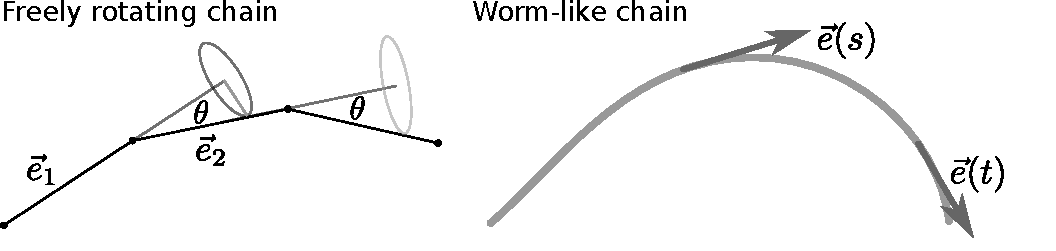
\includegraphics[width=0.96\columnwidth]{figures/stiff_polymers.pdf}
	\caption{{\bf Polymers with stiffness.} The freely rotating chain model (left) assumes that different monomers are at a fixed angle but can rotate freely around the bond. The worm-like chain model is more appropriate for polymer that bend only slightly at individual bonds and where directional changes are occur only after many monomers. The worm-like chain model is characterized by a persistence length that describes the decay in directional correlation between tangent vectors at different positions along the polymer. }
	\label{fig:stiff_polymers}
\end{figure}



\section*{Polymers under force}




\subsection*{Pulling -- optical tweezers}
The 2018 Nobel prize in physics was partly awarded to \href{https://en.wikipedia.org/wiki/Arthur_Ashkin}{Arthur Ashkin} for the development of optical tweezers -- a method to manipulate microscopic objects and measure forces on the pico-newton scale.
In this technique, a focused laser beam traps tiny particles in the center of the focus where the light intensity is highest.
Forces applied to these particle move the trapped particles slightly out of the focus of the beam and diffract light in a way that allows to measure the force applied, see Fig.~\ref{fig:DNA_stretching}.

\begin{figure}[tb]
	\centering
	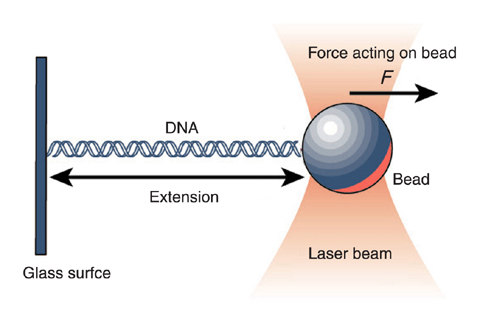
\includegraphics[width=0.6\textwidth]{figures/OpticalTweezers_DNA.png}
	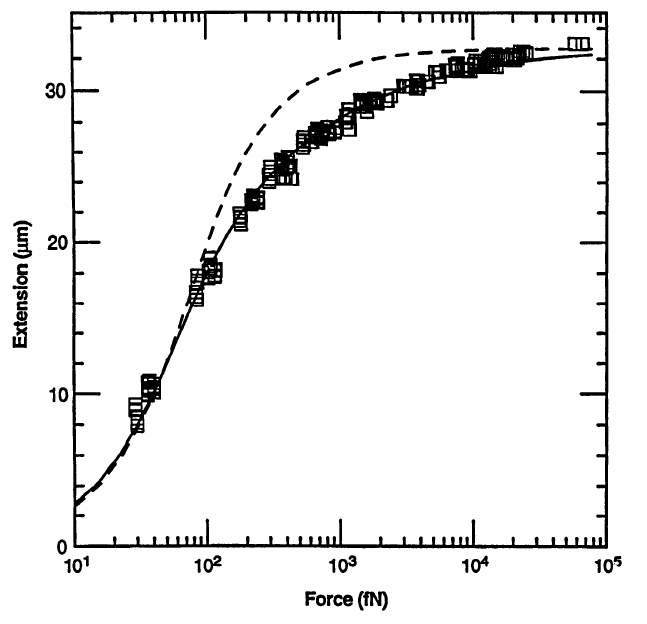
\includegraphics[width=0.39\textwidth]{figures/DNA_force_extension.png}
	\caption{Polymers under force. Left: Schematic representation of an optical tweezer (by \href{http://umdberg.pbworks.com/w/page/47555271}{Joe Redish}). Right: Force-extension curve of double stranded DNA from \cite{bustamante_entropic_1994}.
	The dashed line is the prediction by the freely jointed chain model, the solid line the prediction by the worm-like chain model.}
	\label{fig:DNA_stretching}
\end{figure}

When stretching a flexible polymer, the confirmation changes drastically:
Initially, the polymer is a random coil and the force merely displaces the two end points away from each other.
In this regime, the force generated by the polymer is of ``entropic'' nature.
At higher forces, the end-to-end extension approaches the contour length and the resistance to further extension stems from the elasticity.

\subsubsection*{Entropic springs}

Flexible polymers form random coils and the average end-to-end distance is typically proportional to the square root of the length of the chain.
What happens if you start to pull on the ends? Will it immediately stretch? Or will it act as a spring? How does extension depend on the applied force and the length of the spring?

Let's consider a polymer that consists of segments of length $d$ that are completely freely rotating, i.e., any angle on the sphere is equally likely a priori.
Applying a force will bias this distribution.
The probability of for any given monomer to have an extension $\chi$ is therefore
\begin{equation}
p(\chi|F) = \frac{F}{kT}\frac{e^{F\chi/kT}}{e^{Fd/kT}-e^{-Fd/kT}}
\end{equation}
(this has units $1/length$ as it should.)
The total end-to-end distance in the direction of the force is $x=\sum_i \chi_i$ and the average extension is simply
\begin{equation}
\begin{split}
\langle x \rangle_{F} &= N\int_{-d}^d d\chi \; \chi p(\chi|F) = \frac{FN}{kT(e^{Fd/kT}-e^{-Fd/kT})} \int_{-d}^{d} d\chi \;\chi e^{F\chi/kT} \\
% &= \frac{FN}{kT(e^{Fd/kT}-e^{-Fd/kT})} \int d\chi \; kT \frac{\partial }{\partial F} e^{F\chi/kT} \\
% &= \frac{FN}{e^{Fd/kT}-e^{-Fd/kT}} \frac{\partial }{\partial F}\frac{kT}{F} \left(e^{Fd/kT} - e^{-Fd/kT}\right) \\
% & = \frac{FN}{e^{Fd/kT}-e^{-Fd/kT}} \left(-\frac{kT}{F^2} + d\left(e^{Fd/kT} + e^{-Fd/kT}\right)\right)
& = dN \left(\frac{e^{Fd/kT}+e^{-Fd/kT}}{e^{Fd/kT}-e^{-Fd/kT}} - \frac{kT}{Fd}\right)
\end{split}
\end{equation}
Let's expand this around $F=0$:
\begin{equation}
\langle x \rangle_{F} \approx F\frac{\partial \langle x \rangle_{F}}{\partial F} =  F\frac{d^2N}{3kT}
\end{equation}
Hence to lowest order in $F$ a flexible polymer acts as an entropic spring with spring constant $\frac{3kT}{d^2N}$.
Longer polymers are softer, and increasing temperature makes them stiffer. The smaller the monomers are, the stiffer they are.
This is a well known effect in rubber bands.
Rubber bands are effectively many tightly entangled and cross-linked polymers.
When heated, the flexible bits undergo more vigorous thermal motion resulting in a stronger force resisting extension.
You can find various demonstrations of this effect online, for example \href{https://www.youtube.com/watch?v=eB4B2xZI77A}{in this video}.

\begin{figure}[tb]
	\centering
	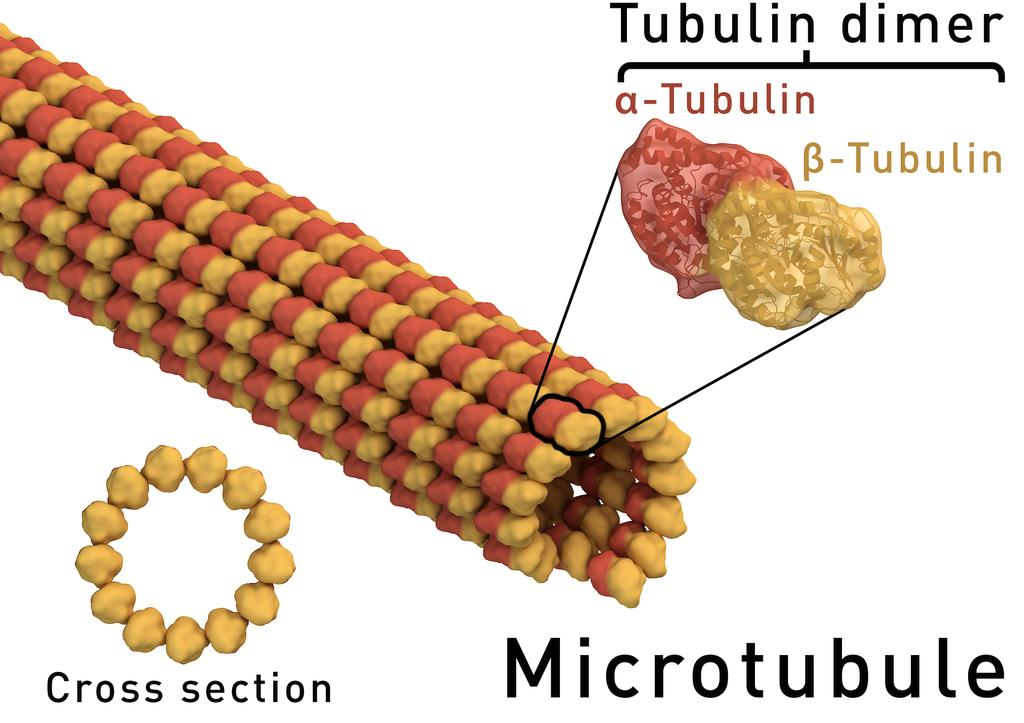
\includegraphics[width=0.35\textwidth]{figures/Microtubule_structure.jpg}
	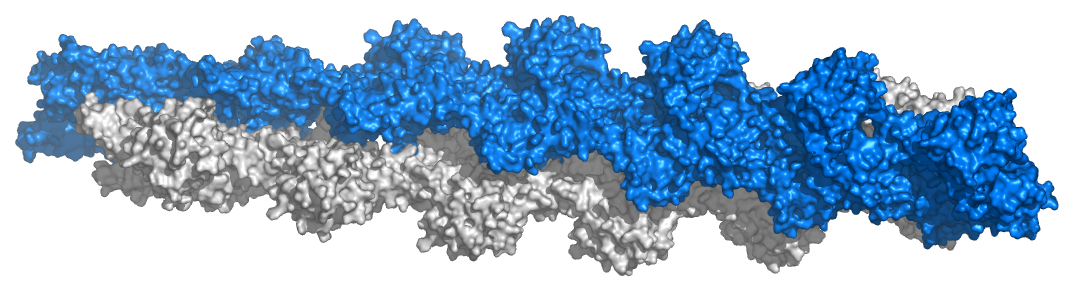
\includegraphics[width=0.62\textwidth]{figures/actin_filament.png}
	\caption{Left: Structure of microtubules. Right: 13 subunit structure of actin filament. Both graphs  are by Thomas Splettstoesser (www.scistyle.com) and retrieved from wikipedia)}
	\label{fig:cytoskeleton_structure}
\end{figure}

A typical RNA molecule with $N=1000$ and $d=2nm$, we would find a spring constant
\begin{equation}
\alpha = \frac{3kT}{d^2N} = \frac{12pN nm}{4nm^2 1000} = 3\times 10^{-3}\frac{pN}{nm}
\end{equation}

In the opposite limit around $x=d$, the behavior of the force extension curve is very different.
\begin{equation}
\langle x \rangle_{F} \approx Nd\left(1 - 2e^{-\frac{Fd}{kT}} + \cdots - \frac{kT}{Fd}\right) \approx Nd\left(1 - \frac{kT}{Fd}\right)
\end{equation}
This implies that at large force $Fd\gg kT$ the polymer is almost completely extended.
Solving this relation for the force yields
\begin{equation}
F = \frac{kT}{d(1- \langle x \rangle/Nd)}
\end{equation}
Hence the force diverges as the polymer approaches full extension.

\begin{figure}[tb]
	\centering
	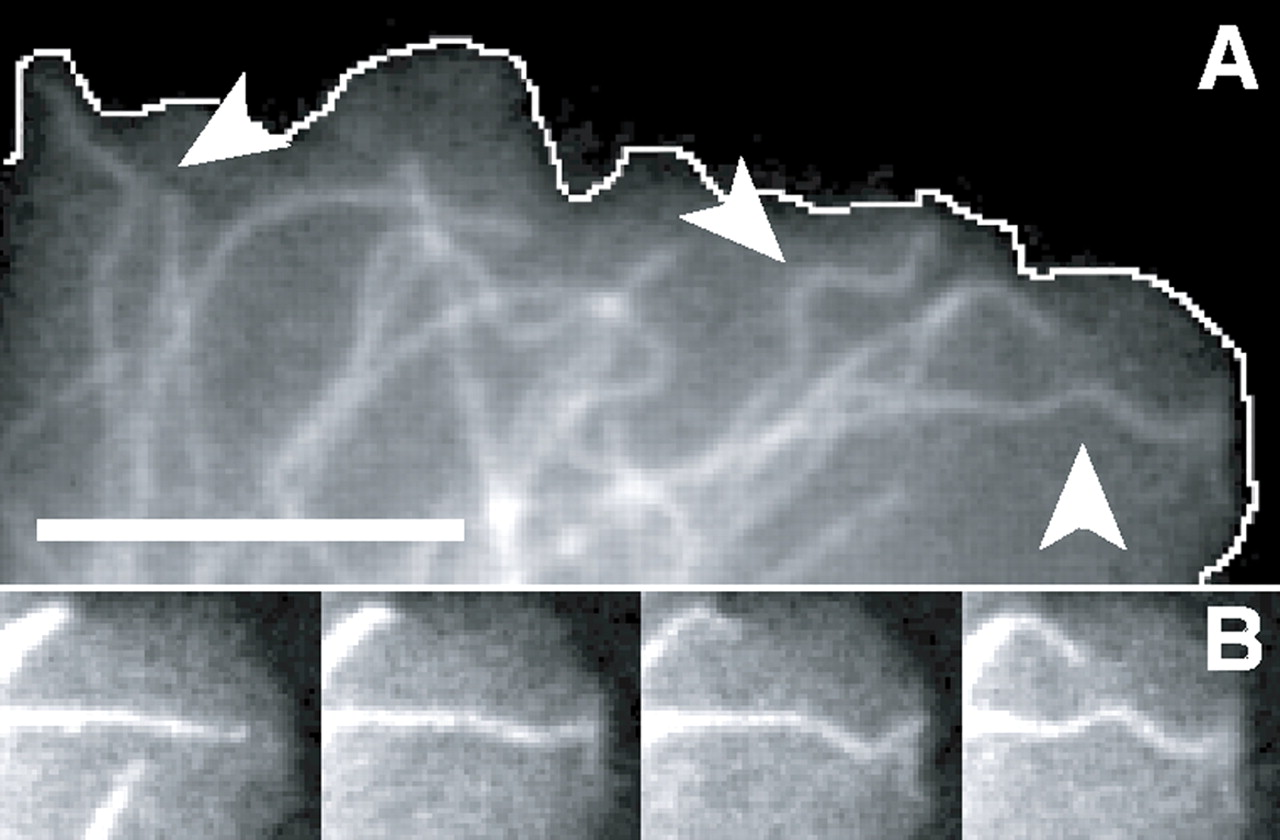
\includegraphics[width=0.5\textwidth]{figures/Brangwynne_microtubule_buckling.jpg}
	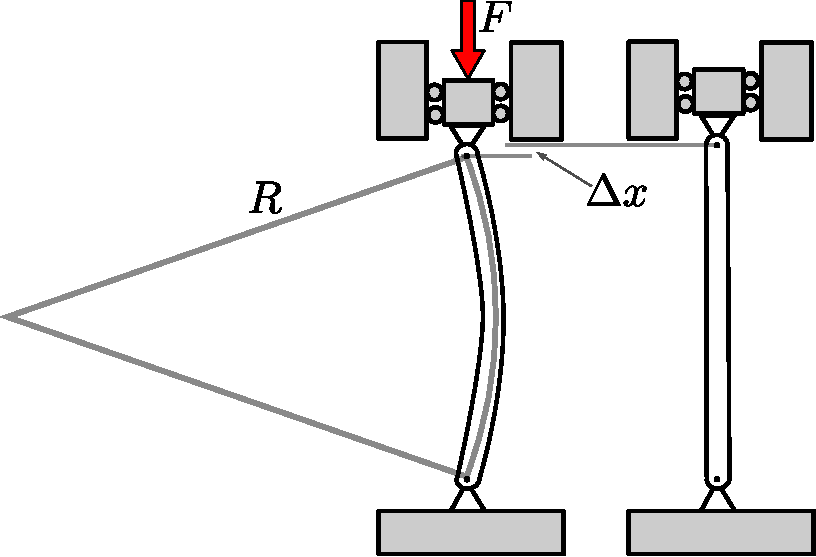
\includegraphics[width=0.48\textwidth]{figures/buckling.pdf}
	\caption{Polymers under force: Buckling of microtubules in cells \citep{brangwynne_microtubules_2006}.}
	\label{fig:buckling}
\end{figure}

\subsection*{Pushing -- buckling instabilities }
If you compress the ends of an elastic rod, it will resist the force until at some point it starts to collapse rapidly.
This is called \emph{buckling}.

How much compressive force can microtubules or other biopolymers withstand before they start to buckle?
Let's write down the energy of a rod of length $L$ when a force $F$ is applied.
When the rod bends, its end-to-end distance gets shorter and the energy of the system is changes do the displacement in the direction of the force (reduction in energy) and the bending of the rod.
The curvature is commonly described by the radius $R$ of the circle that overlaps with the rod's contour.
We will approximate the contour of the rod by an arc of a circle and assume bending is slight, that is the curvature radius $R$ is much bigger than the contour length $L$.
The angle of the arc is $\theta = L/R$ and the end-to-end distance is
\begin{equation}
 x = 2R\sin(L/2R) \approx L - \frac{L^3}{24R^2}
\end{equation}
The displacement in the direction of the force is hence $L^3/24R^2$ and the total energy is
\begin{equation}
E_{tot} = E_{bend} + E_{load} = \frac{\kappa L}{2R^2} + FL(1 - \frac{L^2}{24R^2})
\end{equation}
With increasing curvature (decreasing $R$), the first term increases and the second term decreases.
Whether the total energy increases or decreases depends on the force and parameters of the rod.
We can rewrite the total energy as
\begin{equation}
	E_{tot} = FL + \frac{L}{2R^2}\left[\kappa -\frac{FL^2}{12}\right]
\end{equation}
This tells us that as soon as the force exceeds
\begin{equation}
F_c \approx \frac{12\kappa}{L^2}
\end{equation}
increasing the curvature will further reduce the total energy and the rod will collapse.
At lower forces, the beam

This formula is slightly approximate, since we have assumed that the bent beam is an arc in a circle rather than a sinus curve.
The more accurate calculation would have resulted in $F_c = \frac{\pi^2\kappa}{L^2}$.
But $12$ is close enough to $\pi^2$ for our purpose.
As is intuitively clear, buckling becomes easier when the beam is longer (decreasing with $L^2$) and harder as the material gets stiffer).

To relate this buckling force to cytoskeletal filaments, recall that the persistence length is stiffness $\kappa$ over $kT$ and that $kT$ is $kT\approx 4pN nm$.
The persistence length of microtubules is $\ell_p = 1.4mm$ and a microtubule of length $1\mu m$ has therefore a critical buckling force of
\begin{equation}
	F_c = \frac{12 \ell_p kT}{L^2} = 67 pN
\end{equation}



\subsection*{Force generation through polymerization}
So far, we have assumed the cytoskeletal filaments are fully assembled and static.
This seemed natural -- beams in bridges and building are static after all.
In biology, however, few things are static.
The cytoskeletal filaments are constantly taken apart and repolymerized.
Both microtubuli and actin filaments are polar, meaning they have distinct ends (called minus and plus ends).
The rate at which monomers are added and removed differs between the two ends and incorporation of additional monomers consumes ATP or GTP.

One particularly curious example of force generation through actin polymerization is the propulsion of listeria inside eukaryotic cells.
On one pole the bacterium is decorated with proteins that trigger actin polymerization.
This polymerization pushes the bacterium forward, leaving behind a ``comet tail'' of actin.
Have a look at \href{https://www.youtube.com/watch?v=FIT0fdt6c3Y}{the great video by Julie Theriot} from Stanford University.
Very similar process allow eukaryotic cells to move around or extend filopodia.

\begin{figure}[tb]
	\centering
	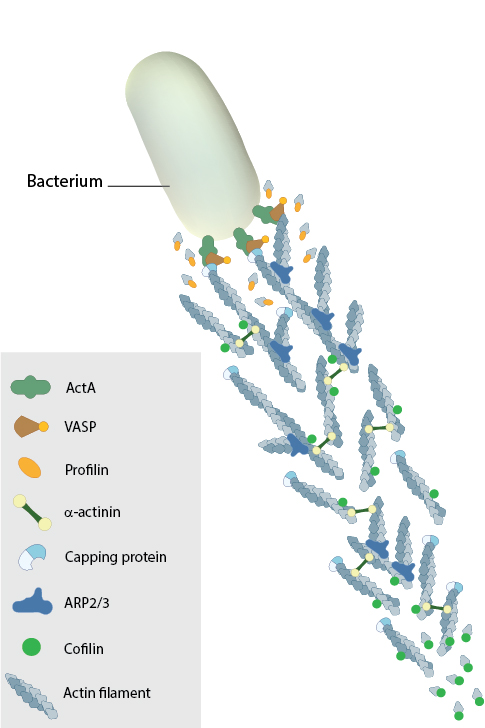
\includegraphics[width=0.38\textwidth]{figures/actin-comet-tails.jpg}
	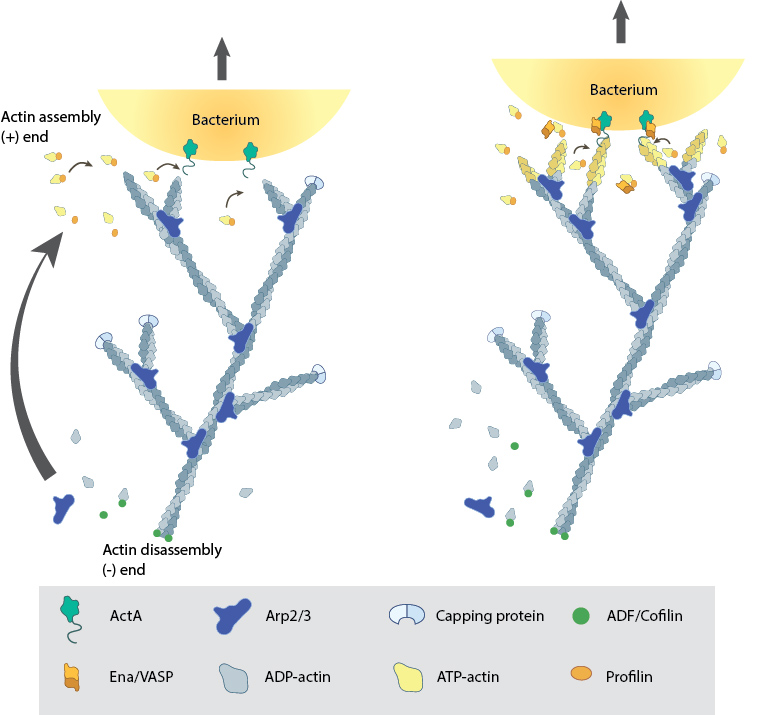
\includegraphics[width=0.61\textwidth]{figures/actin-polymerization-produces-force.jpg}
	\caption{Illustration of actin comet tails and the force generation process from \href{https://www.mechanobio.info/pathogenesis/what-are-actin-comet-tails/}{mechanobio.info}. }
	\label{fig:actin_comet_tail}
\end{figure}


\section*{Self-avoidance, excluded volumes, and self-interaction}
Our discussion of polymers has not considered the fact that a polymer cannot visit a point space that is already occupied by another part of the polymer.
Instead, we have assumed that we can choose the orientation of each monomer regardless of where other monomers are.

It turns out that this is a good approximation in three dimensions, but not in lower dimensions.
In one dimension, this is obvious: if you can only visit points that you have not previously visited, you can never turn back.
In two dimensions, this constraint is less serious, but still substantial: The polymer could never ``cross'' itself. The result is that mean squared end-to-end distances increase more rapidly with the number of monomers $\langle \vec{R}^2\rangle\sim N^{3/2}$ instead of $\sim N$.
In three dimensions, self-avoidance and excluded volume effects only play a small role and $\langle \vec{R}^2\rangle \sim N^{1.17\ldots}$, that is almost linearly in $N$.

In addition to excluded volume effects, self-interactions can affect polymer behavior substantially.
Amino acids in a protein, for example, attract each other (relative to water) and the protein folds into a structure excluding water.
The opposite occurs with DNA. DNA is negatively charged and the charges repel each other.
This results in a stretching of DNA that makes naked DNA stiffer than it would otherwise be.


\section*{DNA looping}
The paradigmatic example of gene regulation -- lactose uptake and processing in E.~coli -- involves a beautiful piece of polymer physics.
To fully repress the lactase operon, two lac repressor dimers have to bind on two location on the DNA and force the DNA into a loop.
The efficiency of repression depends sensitively on the distance between the two binding sites with a periodicity of about 11bp.
This periodicity reflects the helical turn of the DNA: after every turn, the binding sites on the DNA have the right orientation again.


\section{Transcription factor search}
In chapter 2, we discussed the rate at which two molecules encounter each other by diffusion and derived the diffusion limit to association (see Eq.~\ref{eq:diffusion_limit}).
To estimate the rate of transcription factor/DNA association, we can ignore the diffusion of DNA (it is a large slow molecule). Furthermore, the reaction radius should be of the same order as the distance between basepairs since the TFs recognize specific DNA sequences and hence have to be in register with the DNA to 0.3nm. Together with in-vitro measurements of diffusion constant of a transcription factor of about $100\mu m^2/s$, this results in a rate estimate
\begin{equation}
	\kappa_{D} = 4\pi \times 100 \times 3\times 10^{-4} \mu m^3/s \approx 0.4  \mu m^3/s \approx 2\times 10^8 M^{-1}s^{-1}
\end{equation}
However, experiments have shown that the association rate is much higher!
Furthermore, the association rate depends strongly on ionic strength, suggesting that unspecific electro-static interactions help in the binding site search.
This conundrum, and potential solution, is discussed in the review by \citet{hippel_facilitated_1989}.

The basic idea of the mechanisms by which association is sped up is the following:
The TF associates with a random place on the DNA and starts to diffuse along the DNA for a while before detaching again, see Fig.~\ref{fig:TF_search}.
This allows the TF to ``scan'' a section of the DNA in one dimension without having getting lost in 3D.
The problem is hence characterized by a diffusion constant $D_{1D}$ along the DNA in 1D, a diffusion constant $D_{3D}$ in 3D, as well as the average times $\tau_{1D}$ and $\tau_{3D}$ spend in 1D and 3D.


If combined 1D/3D diffusion was the mechanism by which TFs find their target, how should they be dividing their time between 3D and 1D search?
Following \citep{mirny_how_2009}, the total time until the target is found can be expressed as the sum over multiple rounds of 3D/1D search
\begin{equation}
t_s = \sum_{i=1}^K (\tau_{1D,i} + \tau_{3D,i})
\end{equation}
and the typical number of rounds necessary would be $\bar{K} = L/l $ where L is the length of the genome and l is the length searched in a single round.
Since $l\sim \sqrt{2D_{1D} \tau_{1D}}$, we obtain for the average search time
\begin{equation}
 t_s = \frac{L}{\sqrt{2D_{1D} \tau_{1D}} }(\tau_{1D}+\tau_{3D})
\end{equation}
The search time is minimal when
\begin{equation}
 \frac{d t_s}{d \tau_{1D}} = \frac{L}{2\sqrt{2D_{1D}}}(\tau_{1D}^{-1/2}-\tau_{3D}\tau_{1D}^{-3/2}) = 0
\end{equation}
which requires $\tau_{1D} = \tau_{3D}$, i.e., the TF should spend equal times on the DNA and in solution.
The mean search time is therefore
\begin{equation}
 t_s = L\sqrt{\frac{2\tau_{3D}}{D_{1D}}}
\end{equation}

\begin{figure}[tb]
	\centering
	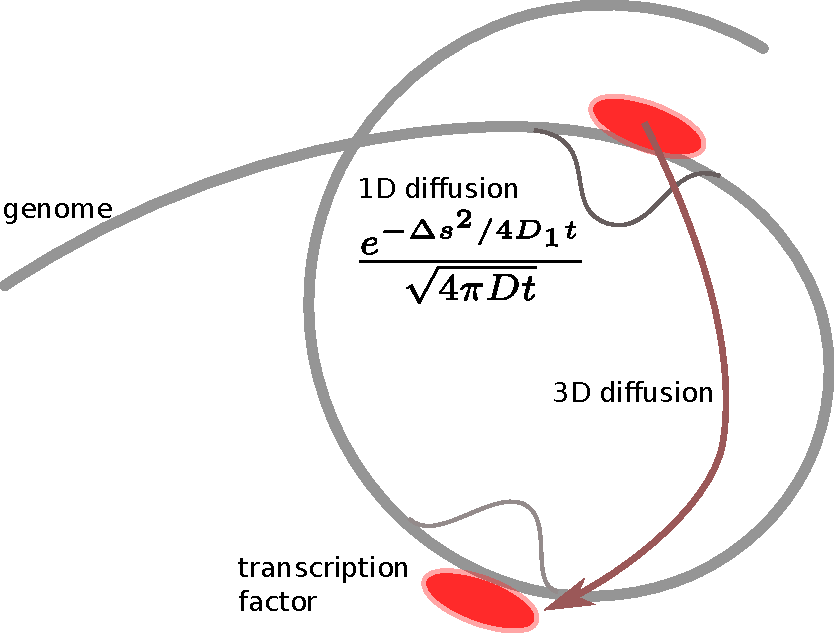
\includegraphics[width=0.7\textwidth]{TF_search.pdf}
	\caption{Illustration of combined 1D/3D search.}
	\label{fig:TF_search}
\end{figure}

\subsection*{Why is there an optimum?}
One dimensional diffusion alone would be extremely inefficient since it takes very long time to scan the entire genome due to the square-root scaling of the distance covered.
Very short $\tau_{1D}$, on the other hand, corresponds to very limited scanning of bases and in the limit of $\tau_{1D}\to 0$ corresponds to pure 3D search.
Hence it is plausible that an optimum should exist.
